%!TEX ROOT = thesis.tex
\chapter{Results and Analysis}

% \section{Data Complexity Analysis}
Prior to the application of our feature selection and resampling methodologies, a detailed analysis of the inherent complexity of each dataset was conducted to provide a foundational understanding of the challenges posed by class imbalance and overlap. The complexity measures of the five classification tasks are presented in Table~\ref{table:data-complexity-tasks}. The measures were calculated based on the development datasets of each classification task.

\begin{table*}[!ht]
    \centering
    \caption{Data complexity measures of different classification and prediction tasks.}
    \begin{tabular}{|p{1.75cm}|l|l|l|l|l|l|l|}
    \hline
       \textbf{Task} & \textbf{Minority Class} & \textbf{IR} & \textbf{Minority \%} & \textbf{F1} & \textbf{kDN} & \textbf{N3} & \textbf{N1} \\ \hline
        NC vs Impaired Classification & Normal & 1.45 & 41\% & 0.975 & 0.245 & 0.3 & 0.49 \\ \hline
        CI vs Dementia Classification & CI & 1.23 & 45\% & 0.98 & 0.268 & 0.324 & 0.505 \\ \hline
        NC vs Impaired Prediction & Impaired & 1.17 & 46\% & 0.98 & 0.246 & 0.304 & 0.526 \\ \hline
        CI vs Dementia Prediction & CI & 1.47 & 40\% & 0.987 & 0.299 & 0.376 & 0.535 \\ \hline
        non-AD vs AD & non-AD & 1.35 & 43\% & 0.996 & 0.351 & 0.429 & 0.596 \\ \hline
    \end{tabular}
    \label{table:data-complexity-tasks}
\end{table*}

The Imbalance Ratio (\acrshort{IR}) and Minority Class Percentage for all tasks indicate a slight to moderate class imbalance, ranging from an IR of 1.17 for the NC vs. Impaired prediction task to 1.47 for the CI vs. Dementia prediction task. The minority class is not severely under-represented in any of the datasets, with the lowest minority percentage being 40\% for the CI vs. Dementia prediction task. This suggests that while imbalance is a factor, it may not be the primary source of difficulty for the classification algorithms.

The complexity is reflected in the feature and neighborhood-based measures. The classification tasks appear to be more significantly influenced by the degree of class overlap. The F1 scores represent the mean of the class separability of each feature. The F1 scores are consistently high, ranging from 0.975 to 0.996. The highest F1 score is observed for the non-AD vs. Alzheimer's (AD) classification task. This indicates a high degree of feature overlap where no single feature can effectively discriminate between AD and other etiologies of cognitive impairment. This underscores the need for a sophisticated feature selection approach to identify a meaningful subset of features.

The neighborhood-based measures, including kDN, N3, and N1, provide crucial insights into the structural and instance-level overlap. The non-AD vs. AD classification task exhibits the highest complexity across these measures (kDN: 0.351, N3: 0.429, N1: 0.596). This suggests that the classes in this task are the most intertwined, with a higher proportion of examples from different classes in a given neighborhood (\acrshort{kDN}), a higher nearest-neighbor error rate (N3), and a more complex decision boundary (N1). The high percentage of borderline examples further supports this, with the minority class (non-AD) having more than half of its instances live in the borderline.

A direct comparison of the current status classification tasks with their corresponding future status prediction tasks reveals a consistent pattern of increased complexity for the predictive models. For the NC vs. Impaired tasks, the prediction task demonstrates slightly higher structural overlap (N1 of 0.526 vs. 0.490) despite a more balanced class distribution (IR of 1.17 vs. 1.45). The same goes for the CI vs. Dementia tasks, whereby the prediction task has higher scores across all overlap measures compared to the CI vs. Dementia classification task. This heightened complexity in the prediction tasks is particularly pronounced in the instance-level and structural overlap metrics, with a higher kDN score (0.299 in prediction task vs. 0.268 for classification) and a more intertwined class structure (N1 of 0.535 vs. 0.505). These findings strongly support the conclusion that predicting a patient's cognitive status five years into the future is a more challenging problem than classifying their current condition.

The results of this complexity analysis provide a clear justification for our ensemble feature selection and resampling methodologies to address the significant class overlap.

\section{Feature Selection}
This section presents the results of our two-step automated feature selection methodology, comparing its performance against a baseline (no feature selection) and the ElasticNet method. The evaluation is based on three key metrics: the number of selected features, the F1 score, and the N3 score, which were then used to calculate a final fitness score. The objective of this comparison is to demonstrate that our method is capable of identifying a more compact and optimal subset of features that concurrently mitigates data complexity, as evidenced by a higher fitness score.

\subsection{Comparative Performance of Feature Selection Methods}
Table~\ref{table:feature-selection-resutls} presents a comprehensive overview of the performance of the three feature selection approaches across all five classification tasks. Our method consistently achieved the highest fitness score in four out of the five tasks, indicating its superior ability to find an optimal balance between reducing data complexity and minimizing the number of selected features. For instance, in the CI vs. Dementia Classification task, our method achieved the highest fitness score of 0.77, outperforming ElasticNet (0.757) and the baseline (0.563). This was accomplished by selecting a compact subset of 12 features, which is significantly fewer than the baseline's 61 features and comparable to ElasticNet's 15. The reduction in the number of features led to a considerable decrease in the N3 score from 0.324 of the baseline to 0.237, which suggests a substantial reduction in class overlap and an easier classification problem.

\begin{table}[!ht]
    \centering
    \caption{Comparison of the feature selection methods' results.}
    \begin{tabular}{|l|l|l|l|l|l|}
    \hline
        Task & Method & \# Features & F1 & N3 & Fitness Score \\ \hline
        \multirow{3}{*}{NC vs Impaired classification} & Ours & 12 & 0.915 & 0.244 & 0.762 \\
        & ElasticNet & 14 & 0.924 & 0.241 & 0.759 \\ 
        & Baseline & 58 & 0.975 & 0.3 & 0.583 \\ \hline
        \multirow{3}{*}{CI vs Dementia classification} & Ours & 12 & 0.926 & 0.237 & 0.77 \\
        & ElasticNet & 15 & 0.947 & 0.242 & 0.757 \\
        & Baseline & 61 & 0.98 & 0.324 & 0.563 \\ \hline
        \multirow{3}{*}{NC vs Impaired prediction} & Ours & 12 & 0.931 & 0.301 & 0.713 \\
        & ElasticNet & 17 & 0.948 & 0.306 & 0.693 \\
        & Baseline & 55 & 0.98 & 0.304 & 0.58 \\ \hline
        \multirow{3}{*}{CI vs Dementia prediction} & Ours & 10 & 0.954 & 0.344 & 0.685 \\
        & ElasticNet & 16 & 0.971 & 0.298 & 0.706 \\
        & Baseline & 58 & 0.987 & 0.376 & 0.52 \\ \hline
        \multirow{3}{*}{non-AD vs AD} & Ours & 12 & 0.991 & 0.403 & 0.631 \\
        & ElasticNet & 16 & 0.992 & 0.405 & 0.619 \\
        & Baseline & 61 & 0.996 & 0.429 & 0.476 \\ \hline
        \multirow{3}{*}{non-AD vs AD (with CDR)} & Ours & 14 & 0.961 & 0.364 & 0.662 \\
        & ElasticNet & 20 & 0.98 & 0.362 & 0.649 \\
        & Baseline & 67 & 0.99 & 0.369 & 0.526 \\ \hline
    \end{tabular}
    \label{table:feature-selection-resutls}
\end{table}

A similar pattern is observed in the other tasks. In the NC vs. Impaired Classification task, our method achieved a fitness score of 0.762 with 12 features, exceeding ElasticNet's score of 0.759 with 14 features. The reduction in the N3 score from 0.300 to 0.244 further highlights the effectiveness of our approach in simplifying the data. The only task where our method was not the best by the fitness score was CI vs. Dementia Prediction. Although ElasticNet scored slightly higher (0.706 vs. 0.685), our method achieved a better F1 score (0.954 vs. 0.971) with a small set of selected features (10 vs. 16). Our methodology's efficacy was further validated by the fact that the Spearman correlation between the rankings from the individual ensemble methods was consistently less than 70\% for all tasks. This low correlation indicates a healthy diversity among the feature selection methods, which is a crucial factor in building a robust and stable ensemble feature selection method.

We observed that feature and instance overlap, as measured by the F1 and N3 scores, remained high for all tasks even after our initial feature selection. This was particularly evident in the non-AD vs. Dementia classification task, which initially showed a high F1 score of 0.991 and an N3 score of 0.403. These results indicated that this specific classification task was very complex and that the classifier would struggle to differentiate the classes using the initial feature set. Therefore, to ease the complexity of class overlap and improve classifier performance, we added clinical dementia rating (CDR) features to the dataset and re-ran the feature selection process for this task. This addition of CDR features resulted in a noticeable improvement. The F1 score for our method decreased from 0.991 to 0.961, and the N3 score decreased from 0.403 to 0.364. This indicates a considerable reduction in class overlap, making the classification problem less difficult. While the number of selected features increased from 12 to 14, the overall fitness score improved from 0.631 to 0.662, demonstrating that the added complexity of a slightly larger feature set was justified by the substantial reduction in class overlap. This finding confirms that feature selection alone is not always a sufficient solution if feature overlap is initially very high. Therefore, integrating features with strong clinical relevance can be a useful way to mitigate the inherent complexities of the data.

\subsection{Analysis of Selected Features}
The features selected by our method across all tasks provide valuable insights into the key indicators of cognitive impairment. The selected features are provided in the appendix. The selection of features associated with behavioral and psychiatric symptoms occurred frequently and consistently. The most frequently selected symptoms were agitation (AGIT), depression (DEPD), anxiety (ANX), apathy or indifference (APA), irritability (IRR), hallucinations (HALL), and delusions (DEL). Additionally, the total score of the Geriatric Depression Scale (NACCGDS) was selected across all tasks, highlighting the strong connection between depression and cognitive impairment. Consistently selecting the total of the functional activity questionnaire (FAQTOTAL) also suggests that a subject's functional abilities on a daily basis are important for both diagnosing and forecasting future cognitive decline. Features from multiple types of assessments are selected for the non-AD vs. AD classification task, with the majority of the features related to the cognitive functions from CDR.

There is an apparent overlap in the selected features when comparing similar tasks. For example, demographic features like the subject's sex (SEX) and years of education (EDUC), as well as several behavioral symptoms were selected for both NC vs. Impaired classification and NC vs. Impaired prediction. These two tasks differ in only one feature. The heart rate (HRATE) was selected for NC vs. Impaired prediction, whereas hallucinations (HALL) was selected for the classification task. Similar overlap can be observed in selected features for CI vs. Dementia classification and prediction tasks.

\section{Data Resampling}
Following our feature selection process, we turn our attention to the use of data resampling. This technique is applied to tackle the issue of class overlap in datasets that also have class imbalance. The specific data resampling methods we chose for each task were guided by the insights we gained from an initial analysis of class overlap measures. The measures of class overlap for each classification task are presented in Table~\ref{table:class-overlap-berfore-data-sampling}. The aim of applying data resampling is to reduce class overlap and improve the model performance on classifying less represented classes. This would eventually lead to better model performance and generalizability. The selected data resampling technique was evaluated using five different classifiers trained using the default hyperparameters. These models include Support Vector Machine (\acrshort{SVM}), Random Forest (\acrshort{RF}), KNN (K-Nearest Neighbor), Logistic Regression (\acrshort{LR}), and Naive Bias (NB). The performance of the models is compared against the other commonly used data resampling techniques, including Random Undersampling (RUS), Random Oversampling (ROS), and Synthetic Minority Oversampling Technique (SMOTE). Stratified cross-validation was used to train the models on resampled data, while validation was done on unresampled data. The results of the data sampling for each classification task are reported in the following subsection.

\begin{table*}[!ht]
    \centering
    \caption{Measures of class overlap used to guide the data sampling for each classification taask}
    \begin{tabular}{|p{2cm}|p{2cm}|l|p{2cm}|p{2cm}|p{2cm}|l|l|}
    \hline
        Task & Minority Class & IR & Overall Borderline Examples & Majority Borderline Examples & Minority Borderline Examples & kDN & N1 \\ \hline
        NC vs Impaired Classification & NC & 1.45 & 24\% & 19\% & 30\% & 0.202 & 0.363 \\ \hline
        CI vs Dementia Classification & CI & 1.23 & 24\% & 22\% & 27\% & 0.202 & 0.373 \\ \hline
        NC vs Impaired Prediction & Impaired & 1.17 & 29\% & 32\% & 25\% & 0.246 & 0.479 \\ \hline
        CI vs Dementia Prediction & CI & 1.47 & 39\% & 29\% & 54\% & 0.295 & 0.42 \\ \hline
        non-AD vs AD classification & non-AD & 1.35 & 37\% & 33\% & 43\% & 0.293 & 0.529 \\ \hline
    \end{tabular}
    \label{table:class-overlap-berfore-data-sampling}
\end{table*}

\subsection{NC vs. Impaired Classification}
The NC vs. Impaired classification task presented a mild class imbalance, with an imbalance ratio of 1.45 and the minority class comprising about 41\% of the data. The data also showed a moderate level of class overlap. The proportion of borderline examples was 24\%, which suggests some ambiguity near the decision boundary. Similarly, the kDN value of 0.202 indicated a noticeable local disagreement, with some instances sitting in mixed neighborhoods. The N1 value of 0.363 also pointed to a moderate global overlap between the classes, meaning there was some intermixing of instances. We understood from these measures that the challenge was not just imbalance but also the complexity and noise within the data. For this reason, we selected a hybrid resampling method, Edited Nearest Neighbor (ENN) coupled with KMeansSMOTE. This approach was chosen to simultaneously address both the moderate level of noise and class overlap and the lack of minority examples.

Edited Nearest Neighbor (ENN) is a considered a data cleaning when it is used to undersample both classes. It works by removing data points from the dataset that are considered noisy or mislabeled. It does this by checking a data point's nearest neighbors. If the majority of a point's neighbors belong to a different class, ENN removes that point. This step helps to clean up the data by removing instances that fall on the wrong side of the decision boundary. Thus, it reduces the noise and class overlap. KMeansSMOTE is an oversampling method. It follows a specific approach instead of randomly generating instances like SMOTE. It uses k-means clustering to group similar minority class instances together and then applies the SMOTE algorithm to generate new synthetic samples only within these specific clusters. This helps to create more meaningful and representative new data points, rather than producing synthetic samples in areas where they might be less helpful. By combining these two techniques, our hybrid method first cleaned the data with ENN and then intelligently created new samples with KMeansSMOTE.

The application of ENN-KMeansSMOTE led to a substantial improvement in data quality and improved model performance as presented in Table~\ref{table:data-resampling-results-task1}. When comparing our method to the baseline with no data resampling, the F1 feature overlap measure was reduced to 0.833, and the N3 class overlap measure was reduced significantly from 0.244 to 0.015. This is a significant reduction in class overlap, showing that the classes became much easier to separate. The F1-score of the classifiers, which measures a balance between precision and recall, remained stable or saw a slight decrease. For example, the F1-score of the LR model remained at 0.847, while for the SVM model, it decreased from 0.851 to 0.846. Most importantly, the selected method was able to effectively improve the recall on the minority class for several models. The RF recall increased from 0.769 in the baseline to 0.810, and KNN recall improved from 0.794 to 0.822. Please refer to Figure~\ref{fig:data-resampling-results-task1}

\begin{table}[!ht]
    \centering
    \caption{Comparison of models' F1-score and class overlap measures (F1 and N3) from different data resampling methods for NC vs Impaired classification task.}
    \begin{tabular}{|l|l|l|l|l|l|l|l|}
    \hline
        Method & SVM & RF & KNN & LR & NB & F1 & N3 \\ \hline
        Baseline & 0.851 & 0.835 & 0.822 & 0.847 & 0.799 & 0.915 & 0.244 \\ \hline
        RUS & 0.835 & 0.834 & 0.809 & 0.83 & 0.797 & 0.902 & 0.22 \\ \hline
        ROS & 0.838 & 0.834 & 0.807 & 0.831 & 0.797 & 0.903 & 0.189 \\ \hline
        SMOTE & 0.838 & 0.836 & 0.811 & 0.832 & 0.799 & 0.902 & 0.202 \\ \hline
        ENN-KMeansSMOTE & 0.846 & 0.845 & 0.82 & 0.847 & 0.838 & 0.833 & 0.015 \\ \hline
    \end{tabular}
    \label{table:data-resampling-results-task1}
\end{table}

\begin{figure}[ht]
    \centering
    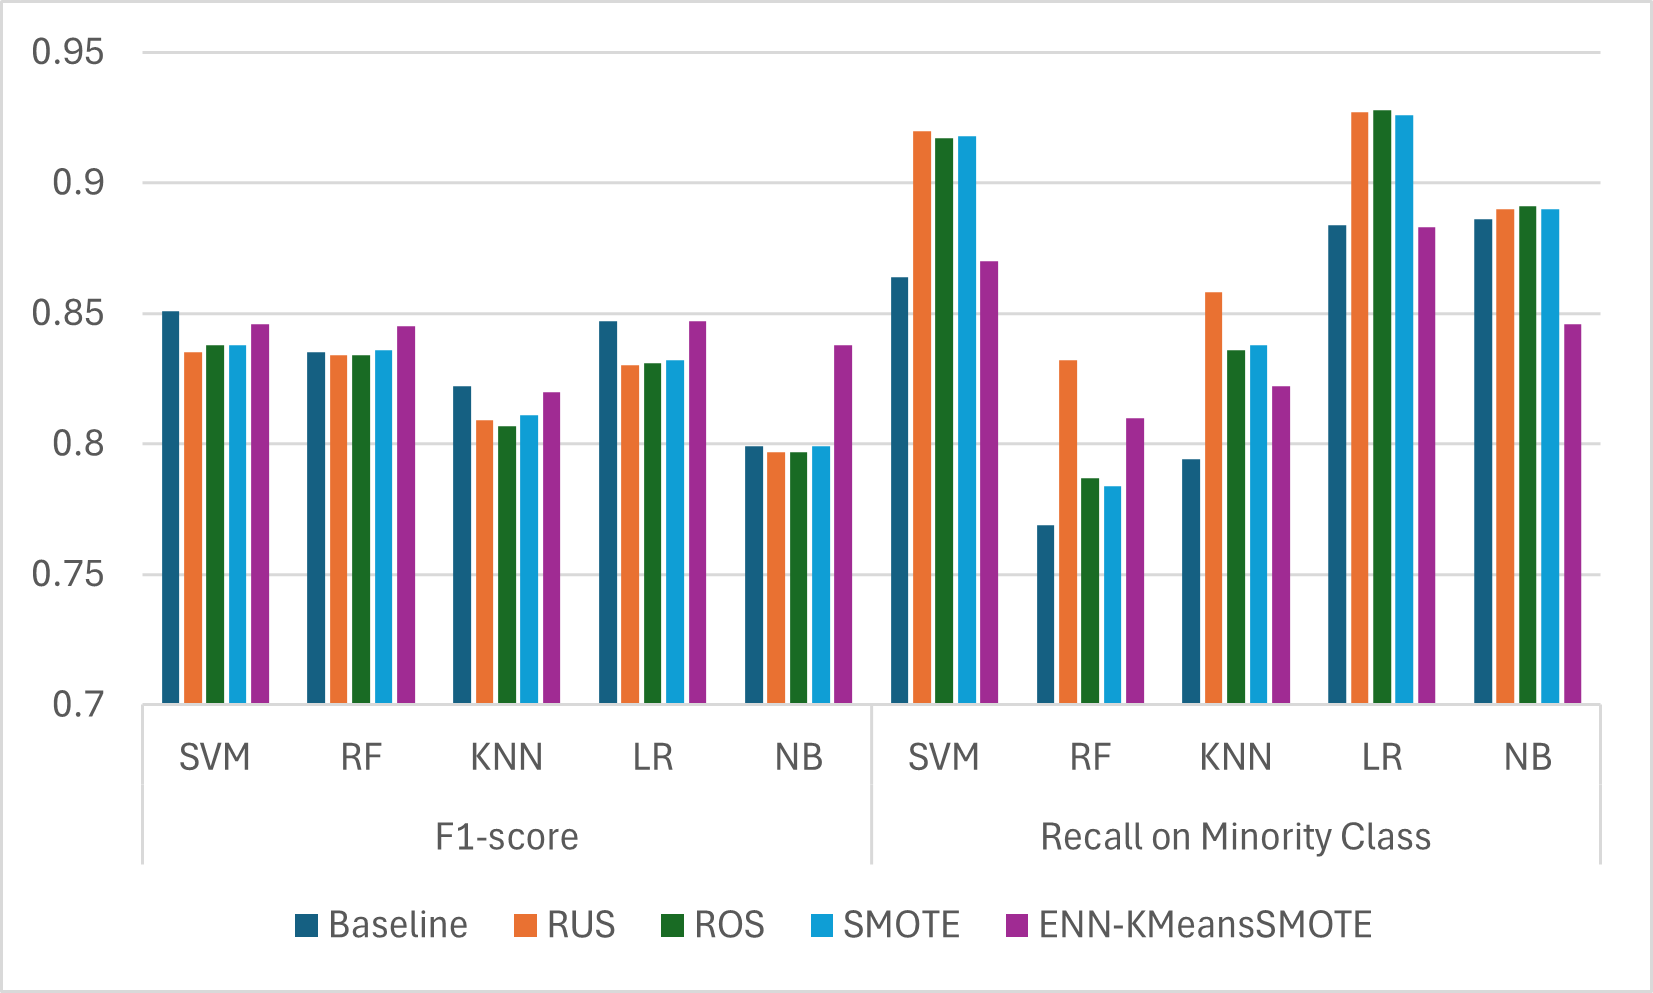
\includegraphics[width=\columnwidth]{figures/ds-task1.png}
    \caption{Comparison of models' F1-score and the recall on minority class from different data resampling methods for NC vs Impaired classification task.}
    \label{fig:data-resampling-results-task1}
\end{figure}

When we compared our method to other common data resampling techniques such as RUS, ROS, and SMOTE, our approach stood out in its ability to reduce class overlap. The ENN-KMeansSMOTE method achieved a much lower N3 score of 0.015, while the other methods had N3 scores of 0.22, 0.189, and 0.202, respectively. This shows that our method was more effective at removing noise and clarifying class boundaries. The other data resampling methods resulted in a higher recall for the minority class. However, they had higher class overlap and lower F1-scores as compared to ENN-KMeansSMOTE. Although the applied data resampling method (ENN-KMeansSMOTE) did not significantly improve the F1-score, it reduced the class overlap and improved the recall on the minority class. This makes the data less complex which can be accurately classified with less complex models.

\subsection{CI vs. Dementia Classification}
The results obtained in this classification task are quite similar to the results of the NC vs. Impaired classification task. The data exhibited a mild class imbalance with an imbalance ratio of 1.23. An analysis of the data's complexity showed a moderate degree of class overlap. The N1 score of 0.373 suggested a meaningful intermixing of the classes. We also noted that the kDN value of 0.202 indicated that many instances were in mixed neighborhoods. Around a quarter of the data samples reside in the class boundaries. This includes 21\% of the majority class and 27\% of the minority class. We concluded from these class overlap measures that applying a hybrid approach of cleaning and oversampling methods may improve the separation between the classes.

Our ENN-KMeansSMOTE approach showed a significant reduction in class overlap when compared to the baseline. A comparison of the data resampling results is provided in Table~\ref{table:data-resampling-results-task2} and Figure~\ref{fig:data-resampling-results-task2}. We observed a substantial drop in the N3 class overlap measure, from 0.237 in the baseline to just 0.018 after applying our method. The F1 feature overlap also decreased from 0.926 to 0.833. The change in these class overlap measures indicates a clearer separation between the classes. However, the recall on the minority class and F1-score were not improved. This can be explained by the high level of feature overlap even after balancing the classes, which could limit the models from making more accurate classifications. Nevertheless, our hybrid method was better at managing class overlap and balancing the classes than RUS, ROS, and SMOTE. These methods achieved slightly higher minority class recalls for some models, but they resulted in lower F1-scores compared to the baseline. This suggests that simply balancing the classes is not sufficient to improve the performance.

\begin{table}[!ht]
    \centering
    \caption{Comparison of models' F1-score and class overlap measures (F1 and N3) from different data resampling methods for CI vs Dementia Classification task.}
    \begin{tabular}{|l|l|l|l|l|l|l|l|}
    \hline
        Method & SVM & RF & KNN & LR & NB & F1 & N3 \\ \hline
        Baseline & 0.843 & 0.828 & 0.818 & 0.84 & 0.789 & 0.926 & 0.237 \\ \hline
        RUS & 0.837 & 0.823 & 0.809 & 0.833 & 0.786 & 0.922 & 0.229 \\ \hline
        ROS & 0.836 & 0.824 & 0.81 & 0.834 & 0.785 & 0.922 & 0.206 \\ \hline
        SMOTE & 0.837 & 0.826 & 0.81 & 0.834 & 0.786 & 0.921 & 0.212 \\ \hline
        ENN-KMeansSMOTE & 0.839 & 0.831 & 0.813 & 0.841 & 0.813 & 0.833 & 0.018 \\ \hline
    \end{tabular}
    \label{table:data-resampling-results-task2}
\end{table}

\begin{figure}[ht]
    \centering
    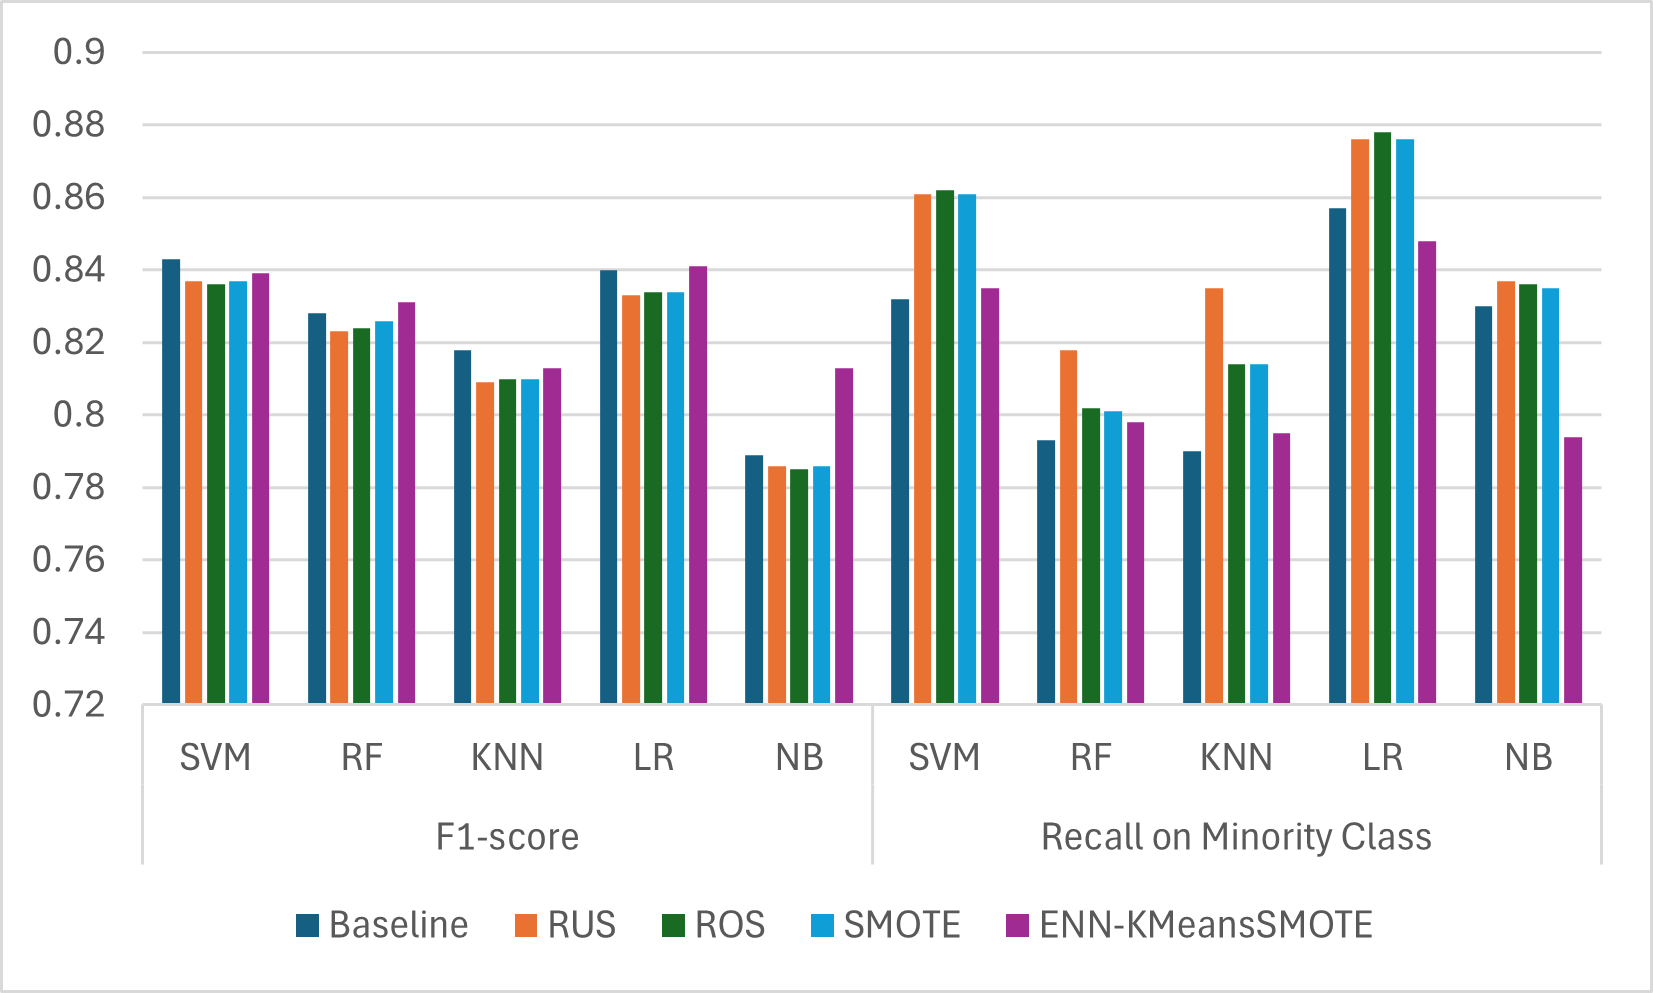
\includegraphics[width=\columnwidth]{figures/ds-task2.png}
    \caption{Comparison of models' F1-score and the recall on minority class from different data resampling methods for CI vs Dementia Classification task.}
    \label{fig:data-resampling-results-task2}
\end{figure}

\subsection{NC vs. Impaired Prediction}
The NC vs. Impaired prediction task showed higher class overlap compared to the previous classification tasks, although the class imbalance is lower, with an imbalance ratio of 1.17. The global overlap, as measured by the N1 score, was 0.479, which points to a strong intermixing of classes, bordering on high overlap. The kDN value of 0.246 and the 29\% overall borderline examples also suggested a moderate level of local noise and ambiguity. Interestingly, a larger proportion of the majority class (32\%) was found at the border compared to the minority class (25\%). To specifically address this high global overlap and the majority class instances crowding the boundary, we chose a new hybrid method: ENN-\acrshort{BorderlineSMOTE}.

The rationale for this selection lies in the way BorderlineSMOTE operates. While both KMeansSMOTE and BorderlineSMOTE generate new data points, BorderlineSMOTE specifically focuses on creating synthetic samples near the decision boundary, where the classes are most difficult to separate. By first applying ENN, we removed noisy examples from both classes, which was a necessary step given the moderate kDN score. After this, BorderlineSMOTE strategically introduced new minority class examples in the critical borderline region, where the model was likely to struggle the most. This two-part strategy was an intelligent way to simultaneously clean up the data and bolster the minority class where it was most needed, as opposed to the clustering-based approach we used for the previous classification tasks.

The results of our ENN-BorderlineSMOTE method were quite promising, as shown in Table~\ref{table:data-resampling-results-task3}. The data structure was significantly improved, with a massive drop in the N3 class overlap measure from 0.303 in the baseline to just 0.013. The F1 feature overlap measure also decreased to 0.896. We also observed an improvement in model performance. The F1-score for most models saw a considerable increase, with SVM going from 0.721 to 0.743 and LR from 0.724 to 0.744, refer to Figure~\ref{fig:data-resampling-results-task3}. More importantly, there was a noticeable gain in recall for the minority class. The recall for SVM increased from 0.613 to 0.712, and for LR, it went from 0.624 to 0.703. This means the classifiers are able to produce more accurate true positives, which is crucial for future prediction of cognitive impairment risk.

\begin{table}[!ht]
    \centering
    \caption{Comparison of models' F1-score and class overlap measures (F1 and N3) from different data resampling methods for NC vs Impaired Prediction task.}
    \begin{tabular}{|l|l|l|l|l|l|l|l|}
    \hline
        Method & SVM & RF & KNN & LR & NB & F1 & N3 \\ \hline
        Baseline & 0.721 & 0.721 & 0.704 & 0.724 & 0.702 & 0.931 & 0.303 \\ \hline
        RUS & 0.729 & 0.725 & 0.707 & 0.735 & 0.705 & 0.934 & 0.308 \\ \hline
        ROS & 0.73 & 0.721 & 0.702 & 0.734 & 0.705 & 0.934 & 0.26 \\ \hline
        SMOTE & 0.729 & 0.719 & 0.706 & 0.734 & 0.705 & 0.935 & 0.266 \\ \hline
        ENN-BorderlineSMOTE & 0.743 & 0.729 & 0.72 & 0.744 & 0.734 & 0.896 & 0.013 \\ \hline
    \end{tabular}
    \label{table:data-resampling-results-task3}
\end{table}

\begin{figure}[ht]
    \centering
    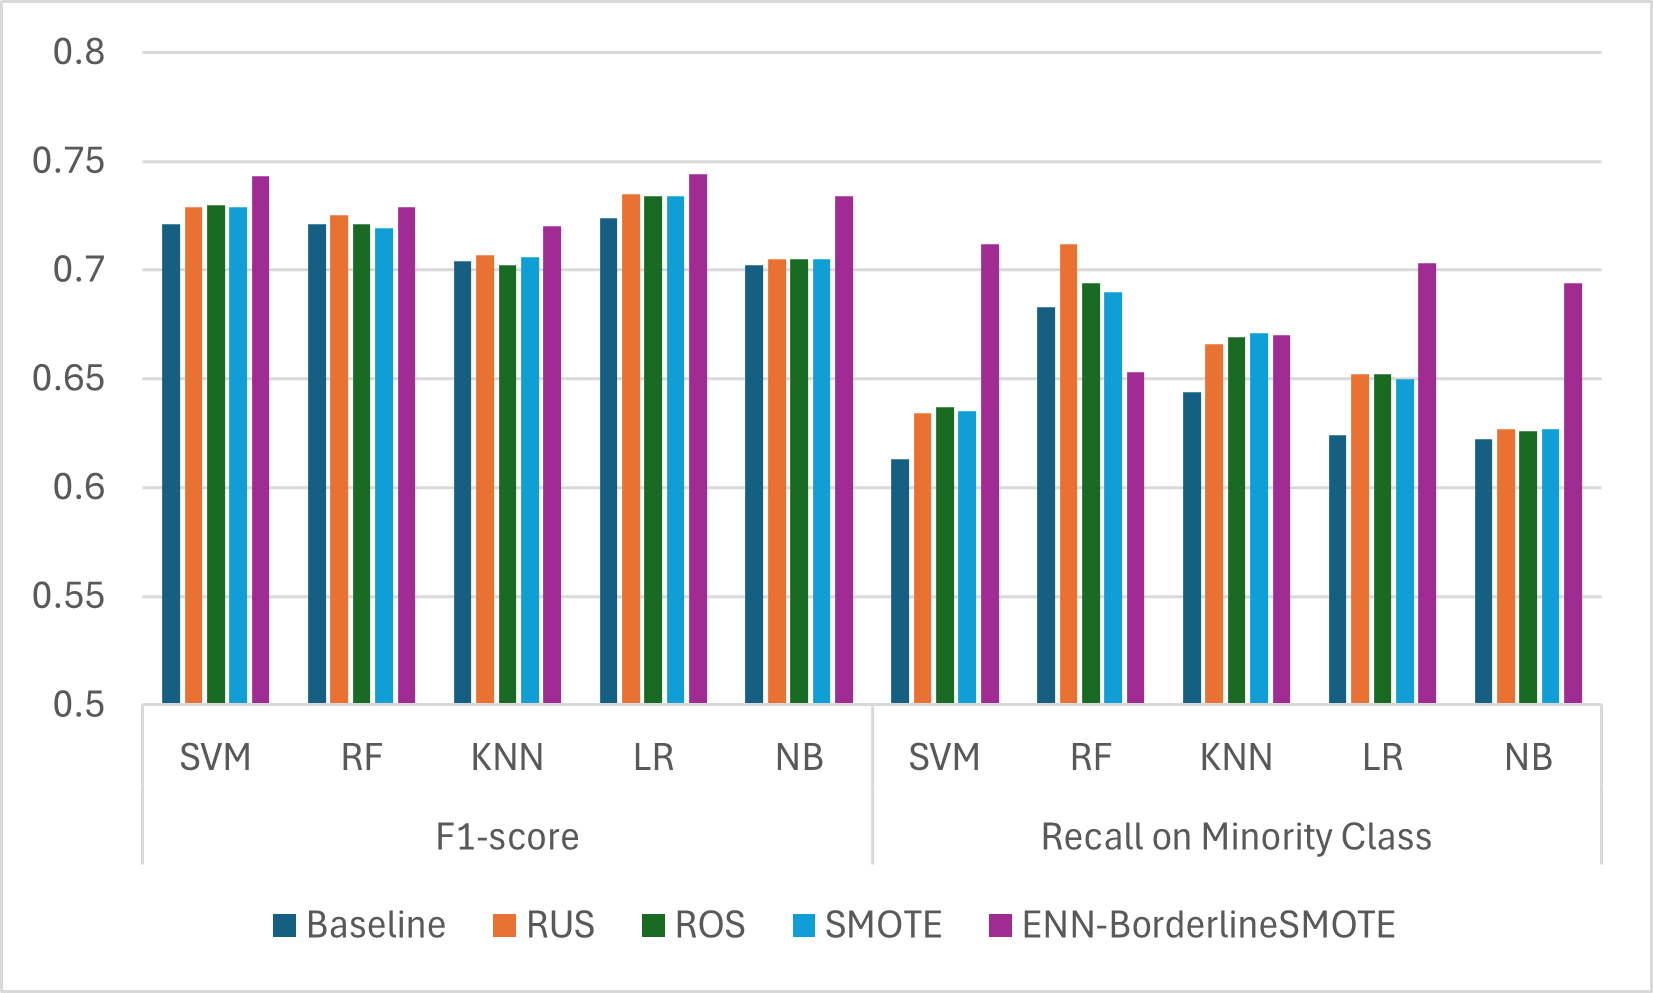
\includegraphics[width=\columnwidth]{figures/ds-task3.png}
    \caption{Comparison of models' F1-score and the recall on minority class from different data resampling methods for NC vs Impaired Prediction task.}
    \label{fig:data-resampling-results-task3}
\end{figure}

The ENN-BorderlineSMOTE method achieved higher F1-scores in all models as compared to the other data resampling methods. While some of these methods did achieve a slight improvement in performance compared to the baseline, they did not manage the underlying data complexity as well as our hybrid approach. Resampling data using these methods resulted in slightly higher F1 feature overlap. This further solidified our belief that balancing classes without handling class overlap may result in more complex data, which impacts the classification performance and limits building generalizable models.

\subsection{CI vs. Dementia Prediction}
The CI vs. Dementia prediction task presented a unique set of challenges compared to the previous classification tasks, although the class imbalance was still mild (IR of 1.47, minority class at 40\%). A high proportion of the examples (39\%) were found near the class boundary, with more than half of the minority class examples residing in this region. The kDN of 0.295 also suggested a substantial level of local noise, and the N1 score of 0.42 pointed to a high global overlap. This combination of factors made the data more difficult to separate. Therefore, we employed a hybrid approach of data resampling, which consists of ENN and Majority Weighted Minority Oversampling Technique (MWMOTE). This method was selected because it combines the noise-reducing capabilities of ENN with a more sophisticated oversampling technique designed to handle highly overlapping data.

MWMOTE is particularly well-suited for this kind of dataset. Unlike the previous oversampling methods we used, MWMOTE does not just create new samples in clusters or at the boundary. Instead, it assigns a weight to each minority example based on how close it is to the majority class. Examples that are deeper within the minority region receive a higher weight, while those at the edge get a lower weight. This selective oversampling helps to both grow the minority class and to effectively push the decision boundary further into the majority class. Our method was an effective way to handle the high level of overlap and boundary issues by first applying ENN to remove noise and then using MWMOTE to strategically create new minority samples.

Our hybrid approach delivered strong results, particularly in improving the underlying data structure and feature overlap. The results are listed in Table~\ref{table:data-resampling-results-task4} and presented in Figure~\ref{fig:data-resampling-results-task4}. This contributed to a significant improvement in minority class recall for the KNN and LR models, which increased from 0.641 to 0.7 and from 0.796 to 0.834, respectively. However, the performance of the other models was decreased. When comparing our method to other approaches like RUS, ROS, and SMOTE, we can see that ENN-MWMOTE was uniquely capable of managing the high level of class overlap. This justifies the higher F1-score achieved by our method in all five models. This further highlights that for datasets with a high proportion of borderline and overlapping examples, a targeted hybrid approach is far more effective than traditional resampling methods.

\begin{table}[!ht]
    \centering
    \caption{Comparison of models' F1-score and class overlap measures (F1 and N3) from different data resampling methods for CI vs Dementia Prediction task.}
    \begin{tabular}{|l|l|l|l|l|l|l|l|}
    \hline
        Method & SVM & RF & KNN & LR & NB & F1 & N3 \\ \hline
        Baseline & 0.788 & 0.764 & 0.755 & 0.79 & 0.757 & 0.954 & 0.344 \\ \hline
        RUS & 0.758 & 0.751 & 0.74 & 0.764 & 0.751 & 0.949 & 0.284 \\ \hline
        ROS & 0.758 & 0.76 & 0.734 & 0.764 & 0.752 & 0.948 & 0.291 \\ \hline
        SMOTE & 0.762 & 0.761 & 0.739 & 0.765 & 0.754 & 0.947 & 0.329 \\ \hline
        ENN-MWMOTE & 0.775 & 0.772 & 0.75 & 0.777 & 0.775 & 0.9 & 0.017 \\ \hline
    \end{tabular}
    \label{table:data-resampling-results-task4}
\end{table}

\begin{figure}[ht]
    \centering
    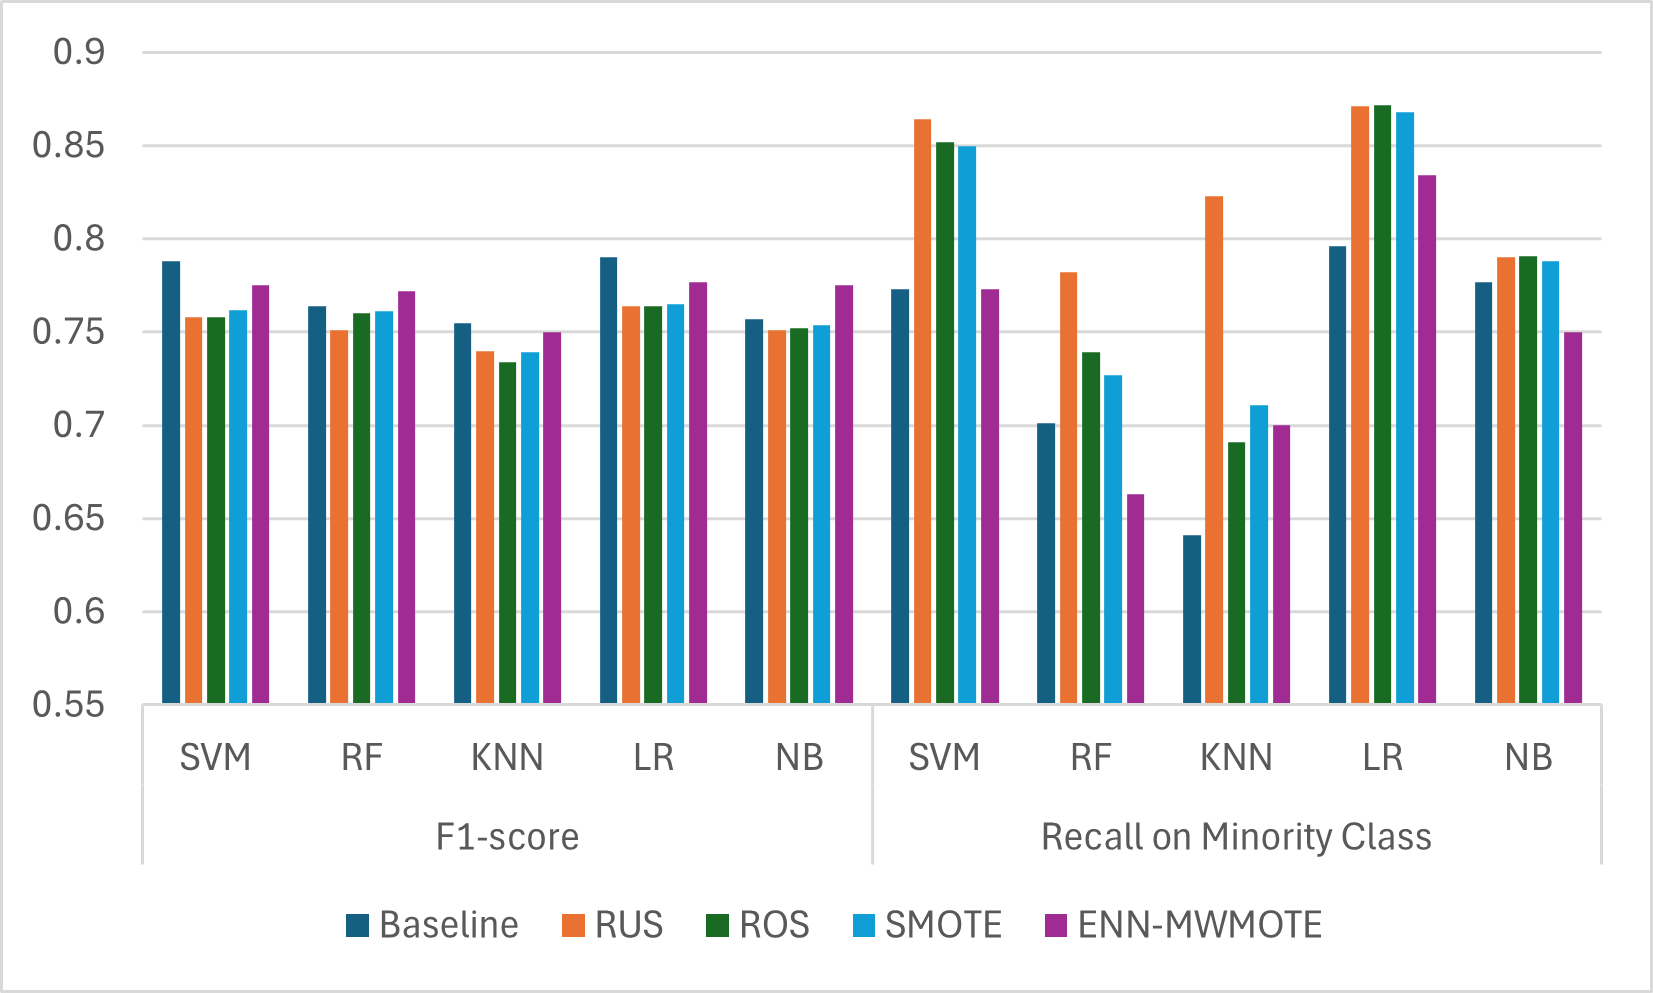
\includegraphics[width=\columnwidth]{figures/ds-task4.png}
    \caption{Comparison of models' F1-score and the recall on minority class from different data resampling methods for CI vs Dementia Prediction task.}
    \label{fig:data-resampling-results-task4}
\end{figure}

\subsection{non-AD vs AD classification}
The non-AD vs. AD classification task had a similar class imbalance, with an IR of 1.35 and the minority class making up 43\% of the data. However, this task presented the most challenging level of class overlap. The N1 score of 0.529 suggests a high degree of global overlap, and the kDN value of 0.293 indicates a significant amount of local noise. 37\% of the overall data were considered borderline examples. The minority class was particularly affected, with a high of 43\% of its instances in the borderline. These measures highlighted a more complex and difficult data structure compared to previous tasks. Given these characteristics, we again selected ENN-MWMOTE as our resampling method. This hybrid approach is designed to handle high class overlap with the need to strategically boost the minority class.

As presented in Table~\ref{table:data-resampling-results-task5}, the application of ENN-MWMOTE showed a clear improvement in the data's underlying structure, highlighted in the decrease of the N3 class overlap measure from 0.364 to 0.032. The F1 feature overlap also decreased from 0.961 to 0.876. In this task we refer to the balanced accuracy instead of the F1 score to reflect our goal of balancing the recall of both AD and non-AD classes. Our method resulted in a considerable increase in accuracy for most models compared to the baseline, refer to Figure~\ref{fig:data-resampling-results-task5}. The highest accuracy increase was in the KNN model, from 0.670 to 0.691. More importantly, the recall on the minority class was significantly improved in all models except RF, with the greatest boost observed in SVM (from 0.675 to 0.742) and LR (from 0.652 to 0.725).

\begin{table}[!ht]
    \centering
    \caption{Comparison of models' Balanced Accuracy and class overlap measures (F1 and N3) from different data resampling methods for non-AD vs AD classification task.}
    \begin{tabular}{|l|l|l|l|l|l|l|l|}
    \hline
        Method & SVM & RF & KNN & LR & NB & F1 & N3 \\ \hline
        Baseline & 0.711 & 0.686 & 0.67 & 0.705 & 0.694 & 0.961 & 0.364 \\ \hline
        RUS & 0.716 & 0.693 & 0.681 & 0.715 & 0.693 & 0.959 & 0.355 \\ \hline
        ROS & 0.716 & 0.686 & 0.67 & 0.715 & 0.694 & 0.96 & 0.288 \\ \hline
        SMOTE & 0.716 & 0.687 & 0.669 & 0.716 & 0.69 & 0.96 & 0.305 \\ \hline
        ENN-MWMOTE & 0.717 & 0.696 & 0.691 & 0.714 & 0.685 & 0.876 & 0.032 \\ \hline
    \end{tabular}
    \label{table:data-resampling-results-task5}
\end{table}

\begin{figure}[ht]
    \centering
    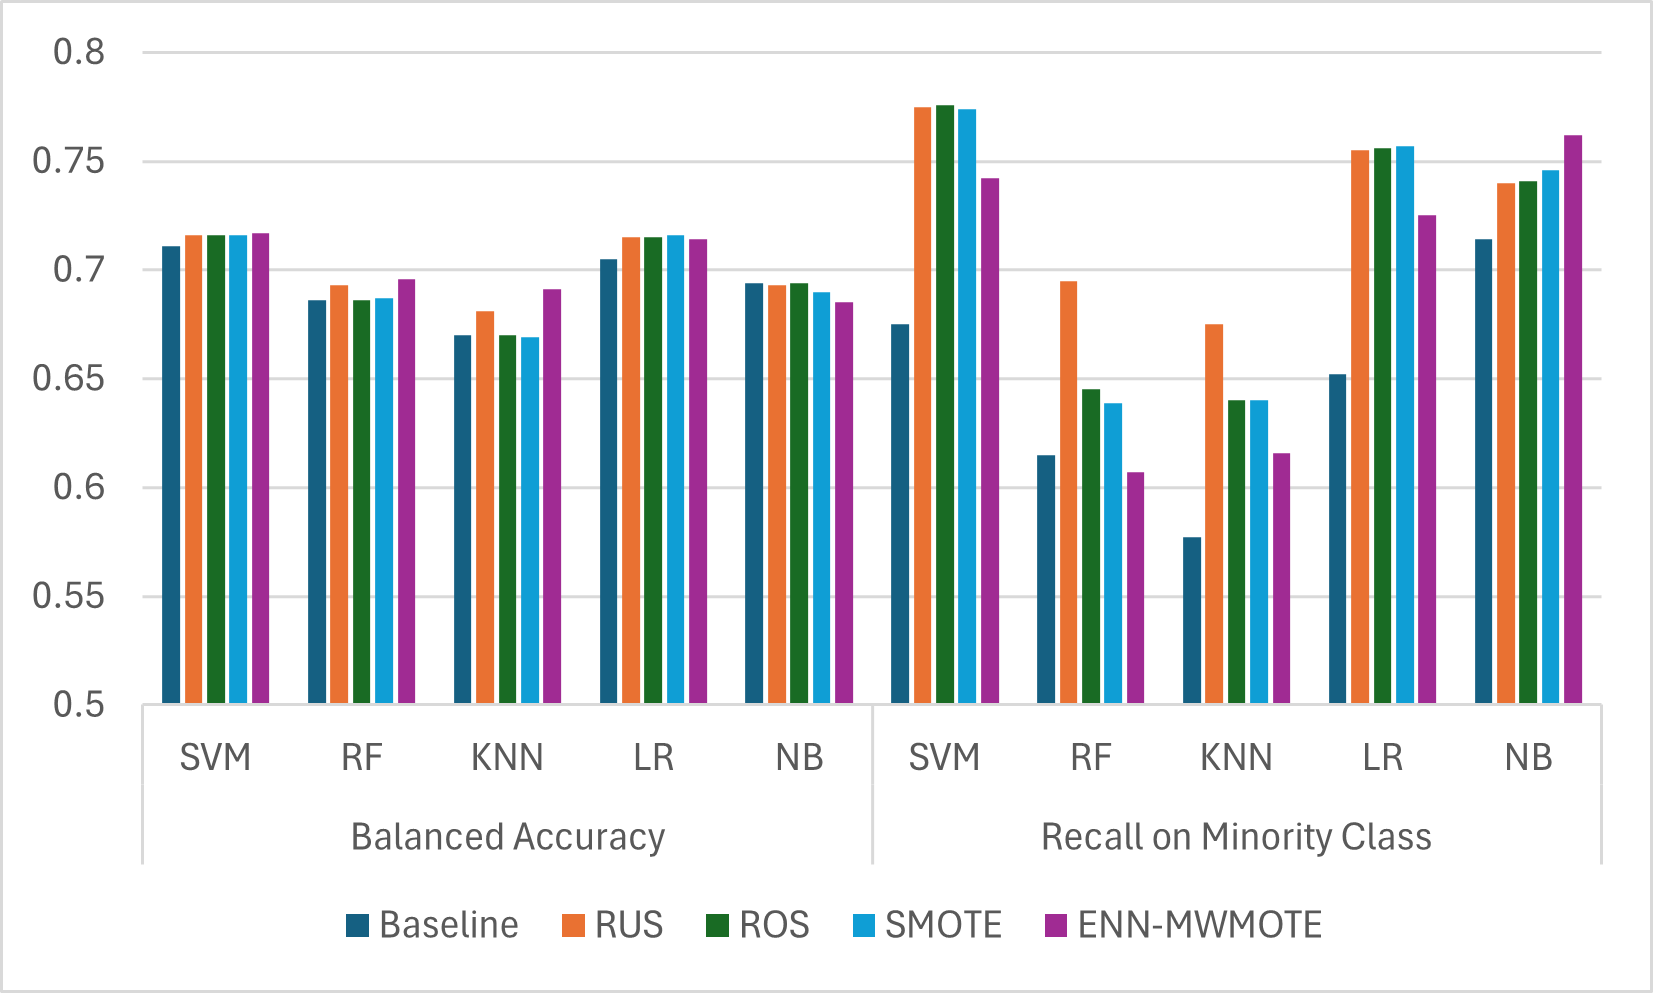
\includegraphics[width=\columnwidth]{figures/ds-task5.png}
    \caption{Comparison of models' balanced accuracy and the recall on minority class from different data resampling methods for non-AD vs AD classification task.}
    \label{fig:data-resampling-results-task5}
\end{figure}

The ENN-MWMOTE method resulted in better accuracy across all models except NB as compared to other data resampling methods. Even though the other methods contributed to better minority class recall, they did not handle class overlap as effectively as ENN-MWMOTE, which could impact the performance of the models in both classes. This reinforces our earlier findings that a targeted hybrid method is a more intelligent and effective way to deal with complex data structures, especially when there is high noise and class overlap.

\subsection{Comparison of Data Resampling Results}
When we looked at the data resampling results across all tasks, a few interesting patterns emerged. First, the reduction in the N3 class overlap score by our chosen methods was remarkable and consistent. The N3 score dropped to a very low level, between 0.013 and 0.032, in all five tasks. This suggests that the hybrid approach of cleaning noisy data with ENN and then strategically oversampling was consistently effective at making the class boundaries much clearer, regardless of the initial data characteristics.

We also noticed a difference between the classification and prediction tasks. The prediction tasks (NC vs. Impaired and CI vs. Dementia) had higher class overlap measures to begin with, and our methods led to a more significant improvement in model performance. For instance, in the NC vs. Impaired prediction, we saw a clear increase in F1-scores and a considerable gain in minority class recall for all models. This was also true for the CI vs. Dementia prediction task, where our method improved the minority class recall for LR and KNN models. In contrast, the classification tasks of the same classes did not see the same level of performance improvement in F1-scores or recall, but they did see a big reduction in class overlap. This suggests that for prediction tasks, addressing class overlap is a more crucial step for improving the model's predictive power.

Looking at the performance of the individual models, we saw that our hybrid methods consistently improved the performance of Logistic Regression and SVM models. These models, especially in the prediction tasks, showed a clear increase in F1-score and minority class recall. The performance of Random Forest and KNN was less consistent, with recall sometimes improving and sometimes decreasing, especially in the non-AD vs. AD task. The performance of the Naive Bayes model also varied, seeing improvements in recall in some tasks but not in others.

Finally, when we compared our methods to the other commonly used techniques (RUS, ROS, and SMOTE), our approach consistently demonstrated a superior ability to reduce class overlap. While the other methods sometimes achieved a higher minority class recall in certain scenarios, they did not manage the underlying data complexity as well, as shown by their higher N3 and F1 class overlap scores. This confirms that our hybrid, two-step approach of first cleaning the data and then strategically oversampling is a more robust and effective strategy for building generalizable models from complex, imbalanced data.

\section{Model Hyperparameter Fine-Tuning}

To fine-tune the hyperparameters of each model, we implemented a grid search with a stratified cross-validation (CV). We used a selection algorithm with predefined criteria to choose the most cost-effective hyperparameters based on the model performance and cost, where the cost is measured by the training and prediction speed.

For the task of classifying normal individuals versus those with cognitive impairment, the RF model and SVM model were the top performers. They both achieved high f1-scores of 0.853 and 0.849, respectively. The LR model also performed very well with a f1-score of 0.848. Incontrast, the KNN model had the lowest f1-score at 0.819. Refer to Table~\ref{table:hyperparameter-resutls-task1}

\begin{table}[!ht]
    \centering
    \caption{NC vs Impaired classification models performance using the selected hyperparameters}
    \begin{tabular}{|l|p{5cm}|l|l|l|}
    \hline
        Model & Selected Hyperparameters & F1-score & Recall & Specificity \\ \hline
        RF & max\_depth = 10.0, max\_features = 'sqrt', min\_samples\_leaf = 6, n\_estimators = 100 & 0.853 & 0.816 & 0.859 \\ \hline
        SVM & C = 10.0, gamma = '0.01', kernel = 'rbf' & 0.849 & 0.804 & 0.87 \\ \hline
        LR & C = 5.0, penalty = 'l2', solver = 'lbfgs' & 0.848 & 0.8 & 0.873 \\ \hline
        KNN & metric = 'euclidean', n\_neighbors = 5, weights = 'distance' & 0.819 & 0.783 & 0.815 \\ \hline
    \end{tabular}
    \label{table:hyperparameter-resutls-task1}
\end{table}

In classifying CI versus dementia, the SVM and RF models again performed the best, with f1-scores of 0.843 and 0.842, respectively. The LR model was close behind with a f1-score of 0.841. The KNN model had a lower f1-score of 0.816. For this task, both SVM and LR models had similar hyperparameter settings to the previous task. Refer to Table~\ref{table:hyperparameter-resutls-task2}

\begin{table}[!ht]
    \centering
    \caption{CI vs Demetnia classification models performance using the selected hyperparameters}
    \begin{tabular}{|l|p{5cm}|l|l|l|}
    \hline
        Model & Selected Hyperparameters & F1-score & Recall & Specificity \\ \hline
        SVM & C = 10.0, gamma = '0.01', kernel = 'rbf' & 0.843 & 0.821 & 0.842 \\ \hline
        RF & max\_depth = 10.0, max\_features = 'log2', min\_samples\_leaf = 6, n\_estimators = 100 & 0.842 & 0.823 & 0.838 \\ \hline
        LR & C = 1.0, penalty = 'l2', solver = 'lbfgs' & 0.841 & 0.817 & 0.844 \\ \hline
        KNN & metric = 'minkowski', n\_neighbors = 3, weights = 'distance' & 0.816 & 0.806 & 0.792 \\ \hline
    \end{tabular}
    \label{table:hyperparameter-resutls-task2}
\end{table}

The task of predicting the transition from normal to impaired cognitive status was more challenging. The RF model achieved the highest f1-score of 0.784. The SVM and LR models also performed well, with f1-scores of 0.782 and 0.778 respectively. The KNN model again had the lowest performance at 0.755. A key trend in this task is that the recall was lower than specificity for both SVM and LR, indicating a better ability to correctly identify the normal class than the impaired class. On the other hand, the RF model had a higher recall than specificity. Refer to Table~\ref{table:hyperparameter-resutls-task3}

\begin{table}[!ht]
    \centering
    \caption{NC vs Impaired prediction models performance using the selected hyperparameters}
    \begin{tabular}{|l|p{5cm}|l|l|l|}
    \hline
        Model & Selected Hyperparameters & F1-score & Recall & Specificity \\ \hline
        RF & max\_depth = 10.0, max\_features = 'sqrt', min\_samples\_leaf = 6, n\_estimators = 100 & 0.784 & 0.769 & 0.715 \\ \hline
        SVM & C = 10.0, gamma = '0.1', kernel = 'rbf' & 0.782 & 0.736 & 0.783 \\ \hline
        LR & C = 5.0, penalty = 'l2', solver = 'lbfgs' & 0.778 & 0.709 & 0.833 \\ \hline
        KNN & metric = 'manhattan', n\_neighbors = 7, weights = 'uniform' & 0.755 & 0.73 & 0.699 \\ \hline
    \end{tabular}
    \label{table:hyperparameter-resutls-task3}
\end{table}

Classifying dementia cases from cognitive impairment cases was similar to the previous prediction task. The performance metrics were lower than the classification tasks. The RF model had the highest f1-score of 0.752. The SVM model also performed well with an f1-score of 0.751. The LR model achieved a f1-score of 0.747, and KNN had the lowest score at 0.733. The selected hyperparameters for RF, SVM, and KNN were similar to the settings in other tasks. However, the LR model used a lower C value of 0.01. Refer to Table~\ref{table:hyperparameter-resutls-task4}

\begin{table}[!ht]
    \centering
    \caption{CI vs Dementia prediction models performance using the selected hyperparameters}
    \begin{tabular}{|l|p{5cm}|l|l|l|}
    \hline
        Model & Selected Hyperparameters & F1-score & Recall & Specificity \\ \hline
        RF & max\_depth = 10.0, max\_features = 'sqrt', min\_samples\_leaf = 6, n\_estimators = 100 & 0.752 & 0.726 & 0.823 \\ \hline
        SVM & C = 10.0, gamma = 'scale', kernel = 'rbf' & 0.751 & 0.718 & 0.833 \\ \hline
        LR & C = 0.01, penalty = 'l2', solver = 'lbfgs' & 0.747 & 0.713 & 0.832 \\ \hline
        KNN & metric = 'minkowski', n\_neighbors = 9, weights = 'uniform' & 0.733 & 0.688 & 0.837 \\ \hline
    \end{tabular}
    \label{table:hyperparameter-resutls-task4}
\end{table}

Classifying non-AD vs. AD was the most difficult task for all models. The SVM and LR models were the top performers, with geometric mean (\acrshort{G-mean}) scores of 0.717 and 0.714 respectively. The RF model had a G-mean of 0.711, while the KNN model's G-mean was significantly lower at 0.68. For this task, the LR model's hyperparameters included a very low with C value of 0.1. This is an indication of the complexity of the data in this task, as the models required strong regularization to perform well. Refer to Table~\ref{table:hyperparameter-resutls-task5}

\begin{table}[!ht]
    \centering
    \caption{Non-AD vs AD classification models performance using the selected hyperparameters}
    \begin{tabular}{|l|p{5cm}|l|l|l|}
    \hline
        Model & Selected Hyperparameters & G-mean & Recall & Specificity \\ \hline
        SVM & C = 10.0, gamma = '0.01', kernel = 'rbf' & 0.717 & 0.68 & 0.756 \\ \hline
        LR & C = 0.1, penalty = 'l2', solver = 'lbfgs' & 0.714 & 0.702 & 0.725 \\ \hline
        RF & max\_depth = 10.0, max\_features = 'sqrt', min\_samples\_leaf = 1, n\_estimators = 100 & 0.711 & 0.747 & 0.677 \\ \hline
        KNN & metric = 'minkowski', n\_neighbors = 3, weights = 'distance' & 0.68 & 0.769 & 0.6 \\ \hline
    \end{tabular}
    \label{table:hyperparameter-resutls-task5}
\end{table}

The proposed cost-effective model selection algorithm makes selecting the proper model hyperparameter values more convenient, even for individuals with a limited understanding of the machine learning algorithms. Researchers and developers can translate their unique performance and cost requirements as parameter values of the selection algorithm to select hyperparameters that meet their business use case needs. This makes the cost-effective model selection algorithm useful for use cases with limited professional resources aiming to develop the best cost-performance models. This aligns with our research objective to make dementia prediction accessible to people in low and middle-income countries (LMICs).

The flexibility of user-defined parameters makes the cost-effective model selection algorithm adaptable to diverse use cases beyond dementia risk prediction. The algorithm particularly benefits businesses operating in an environment where a balance between performance and cost is crucial. For instance, real-time decision-making is essential in safety-critical industries like manufacturing. Similarly, it is cost-effective to frequently update financial models with the latest fraud patterns, using minimum resources and within the shortest possible turnaround time. The cost saving of using efficient models with fast prediction speed becomes evident in applications that require deploying the model in cloud infrastructure, where the cost of operating the model as a service is determined by the resources necessary to operate the model and the required time to serve model inference requests. In most cases, the high cost of building and operating machine learning models is transferred to end users, making the models widely inaccessible. This is where the proposed selection algorithm serves its purpose by reducing the complexity of model fine-tuning, allowing businesses, researchers, and engineers to build solutions at lower costs and make them available to diverse users.

The proposed cost-effective model selection algorithm exhibits more notable advantages regarding its practical use. The algorithm's structured three-phase approach emerges as a pivotal strength, streamlining the complex model selection process and amplifying clarity and implementation ease. This structured implementation enhances the algorithm's transparency and facilitates comprehension for both technical and non-technical users. Another advantage lies in the algorithm's adaptability to various performance metrics, making it flexible and versatile in different industries. Importantly, the algorithm's phased structure and user-friendly parameter customization make it accessible to a broad audience, bridging the gap between domain experts and engineers. Moreover, the algorithm's ease of integration into existing machine learning pipelines further solidifies its practical utility, positioning it as a valuable tool for business and academic applications.

After discussing the advantages of the cost-effective model selection algorithm, it is fair to note its limitations. The algorithm requires the training and prediction throughputs of the models to be measured, which is not a common process of model development. Another limitation of the proposed selection algorithm is its high dependence on the accuracy of the parameter values. Therefore, a nuanced understanding of business requirements is necessary to ensure the algorithm's success. To address this challenge, researchers could explore developing guidelines or tools that assist users in determining appropriate parameter values based on their unique contexts. Additionally, the algorithm may encounter difficulties in scenarios where specific business objectives are not easily quantifiable, such as model interpretability and ethical considerations. Future investigations might explore enhancing the algorithm to incorporate qualitative reasoning approaches. Finally, it is essential to note that the algorithm only uses the model speed to measure the cost of the model. Incorporating other metrics, such as the number of consumed hardware resources, may be useful for specific use cases.

\section{Model Fintuning and Selection}

After fine-tuning the hyperparameters and selecting the best combinations of hyperparameter values for each model, we spot-checked the classification models to select the best model that aligns with our research objectives. We compared the models based on their performance, efficiency, and interpretability, in predicting cognitive impairment in an early stage. To compare the speed of the models, the median training and prediction time of each model was calculated from the training and prediction time recorded during CV. We used the median figures to calculate the training and prediction throughput across all CV iterations. It is worth noting that the models' efficiency in this study is only measured based on the training and prediction speed. However, incorporating additional metrics, such as memory consumption, may provide a more comprehensive perspective for assessing the efficiency of the classification models. According to the results, KNN is a lazy learning algorithm that does not perform any explicit training. Instead, it simply memorizes the training data and makes predictions based on the similarity between the new input data and the training data. This allows the KNN model to record the highest training speed compared to other evaluated models. Similarly, the logistic regression model provides a high prediction speed, as it uses a computationally efficient linear transformation of input features. The random forest models also recorded considerable prediction throughputs due to their ensemble nature. During prediction, this ensembles efficiently aggregate the predictions of base estimators, leading to faster prediction than other complex models. The prediction of SVM models involves computing the decision boundary in a high-dimensional space, making predictions computationally intensive, especially when dealing with large feature spaces or complex decision boundaries.

The interpretability of model output is essential in ensuring the effectiveness of machine learning models for both personal and clinical use \cite{Khan2021Machine}. To further compare the available classification models, we categorized them into three interpretability categories: interpretable, less interpretable, and black-box models. Logistic regression and KNN models are categorized as interpretable models due to their simple and transparent decision-making processes that are directly translatable into human-understandable rules and relationships between features and predictions. Less interpretable models consist of the ensemble models, including the random forest and XGBoost models. Although the prediction of a single base estimator of these ensemble models can be separately interpreted, the contribution of each base estimator to the final prediction is less interpretable. We classified the SVM with RBF kernel as black-box model. Understanding the logic behind the prediction of this model is difficult because of their complex internal structure and decision-making approach. We observed that SVM achieved superior performance but at the cost of lower training and prediction speed than other models. The complexity of a model affects its overall performance, speed, and interpretability. As model complexity increases, performance improves, but speed and interpretability decrease. Conversely, simple models with low performance, such as logistic regression, are fast and easy to interpret.  

After discussing the performance, speed, and interpretability of the available models, selecting a suitable model depends on the unique requirements of the model use case. Concerning our research objectives, we have determined that the RF and LR model are the most suitable for developing a low-cost, accessible, and accurate cognitive impairment prediction solution. They are the best models to balance performance and cost as it offers competent performance with considerable training and prediction speed even on low-cost hardware resources. It has been observed that RF models are widely employed for Alzheimer's disease detection due to their interpretability and robustness.

\section{External Validation}
The generalizability of our models was tested on an unseen dataset from the NACC database and an external dataset from the ADNI database (ADNI test). The performance of the two selected models, Random Forest (RF) and Logistic Regression (LR), was compared across five tasks to understand their ability to generalize.

\subsection{Performance Across NACC Research Centers}
The RF and LR models demonstrated strong and comparable performance across all tasks on the NACC test set. Refer to Table~\ref{table:nacc-test-results} for complete results. The classification tasks, specifically NC vs. Impaired and CI vs. Dementia, showed the highest F1-scores and G-means, ranging from 0.813 to 0.835. This suggests that the models found these problems easier to solve due to the distinct nature of the classes at the time of the patient's visit. For the NC vs. Impaired classification, both models achieved an F1-score of 0.827. In the CI vs. Dementia classification, the RF model had a slightly higher F1-score (0.835) than the LR model (0.834), while their G-means were nearly identical.

\begin{table}[!ht]
    \centering
    \caption{The performance of RF and LR models on NACC test across different research centers}
    \begin{tabular}{|l|l|l|l|l|l|}
    \hline
        Task & Model & F1-score & G-mean & Recall & Specificity \\ \hline
        \multirow{2}{*}{NC vs Impaired Classification} & RF & 0.827 & 0.813 & 0.83 & 0.796 \\
        ~ & LR & 0.827 & 0.816 & 0.818 & 0.813 \\ \hline
        \multirow{2}{*}{CI vs Dementia Classification} & RF & 0.835 & 0.829 & 0.857 & 0.801 \\
        ~ & LR & 0.834 & 0.829 & 0.849 & 0.81 \\ \hline
        \multirow{2}{*}{NC vs Impaired Prediction} & RF & 0.738 & 0.768 & 0.736 & 0.8 \\
        ~ & LR & 0.751 & 0.779 & 0.756 & 0.802 \\ \hline
        \multirow{2}{*}{CI vs Dementia Prediction} & RF & 0.777 & 0.73 & 0.789 & 0.675 \\
        ~ & LR & 0.794 & 0.786 & 0.738 & 0.838 \\ \hline
        \multirow{2}{*}{non-AD vs Dementia} & RF & 0.729 & 0.687 & 0.734 & 0.643 \\
        ~ & LR & 0.724 & 0.704 & 0.696 & 0.712 \\ \hline
    \end{tabular}
    \label{table:nacc-test-results}
\end{table}

The prediction tasks, however, proved more challenging, as evidenced by lower performance metrics. The NC vs. Impaired prediction task resulted in F1-scores of 0.738 for RF and 0.751 for LR. The CI vs. Dementia prediction task had F1-scores of 0.777 for RF and 0.794 for LR. The difference in performance between classification and prediction tasks is expected because predicting future outcomes is inherently more difficult than classifying current conditions. It is interesting to note that in the prediction tasks, the LR model generally achieved slightly higher F1-scores and G-means, suggesting it may be better at identifying long-term trends in the data.

The non-AD vs. AD classification task was the most difficult, with both models achieving the lowest F1-scores (RF at 0.729, LR at 0.724). This is likely due to the highly nuanced differences between these two conditions, which can lead to more overlap in the data.

\subsection{Performance on ADNI Test Set}
We observed a slightly different results when we tested the models on the external ADNI dataset, refer to Table~\ref{table:adni-test-results} . For the classification tasks, the NC vs. Impaired classification model showed high performance, with an F1-score of 0.855 for RF and 0.848 for LR. In this case, the specificity (RF: 0.912, LR: 0.936) was notably higher than the recall (RF: 0.773, LR: 0.756), suggesting that the models were very good at correctly identifying healthy individuals but struggled more with identifying those with cognitive impairment. For the CI vs. Dementia classification, the models performed well, with F1-scores of 0.803 (RF) and 0.802 (LR). The recall and specificity for this task were more balanced compared to the other classification tasks.

\begin{table}[!ht]
    \centering
    \caption{The performance of RF and LR models on ADNI test data.}
    \begin{tabular}{|l|l|l|l|l|l|}
    \hline
        Task & Model & F1-score & G-mean & Recall & Specificity \\ \hline
       \multirow{2}{*}{NC vs Impaired Classification} & RF & 0.855 & 0.84 & 0.773 & 0.912 \\
        ~ & LR & 0.848 & 0.841 & 0.756 & 0.936 \\ \hline
        \multirow{2}{*}{CI vs Dementia Classification} & RF & 0.803 & 0.858 & 0.87 & 0.847 \\
        ~ & LR & 0.802 & 0.855 & 0.849 & 0.862 \\ \hline
        \multirow{2}{*}{NC vs Impaired Prediction} & RF & 0.773 & 0.775 & 0.688 & 0.874 \\
        ~ & LR & 0.771 & 0.778 & 0.672 & 0.902 \\ \hline
        \multirow{2}{*}{CI vs Dementia Prediction} & RF & 0.69 & 0.759 & 0.763 & 0.754 \\
        ~ & LR & 0.686 & 0.754 & 0.692 & 0.822 \\ \hline
    \end{tabular}
    \label{table:adni-test-results}
\end{table}

The prediction tasks on the ADNI dataset had lower performance, similar to the NACC test results. For NC vs. Impaired prediction, the F1-scores were 0.773 for RF and 0.771 for LR. The CI vs. Dementia prediction task resulted in the lowest scores, with F1-scores of 0.690 for RF and 0.686 for LR. This reinforces the conclusion that prediction is the more challenging task.

\subsection{Comparison Between NACC and ADNI Test Results}
We compared the performance of the models on the NACC and ADNI test sets to assess how well the models could accurately classify data from different settings. In general, the models demonstrated high generalizability. Refer to Figure~\ref{fig:nacc-adni-test-compare}

\begin{figure}[ht]
    \centering
    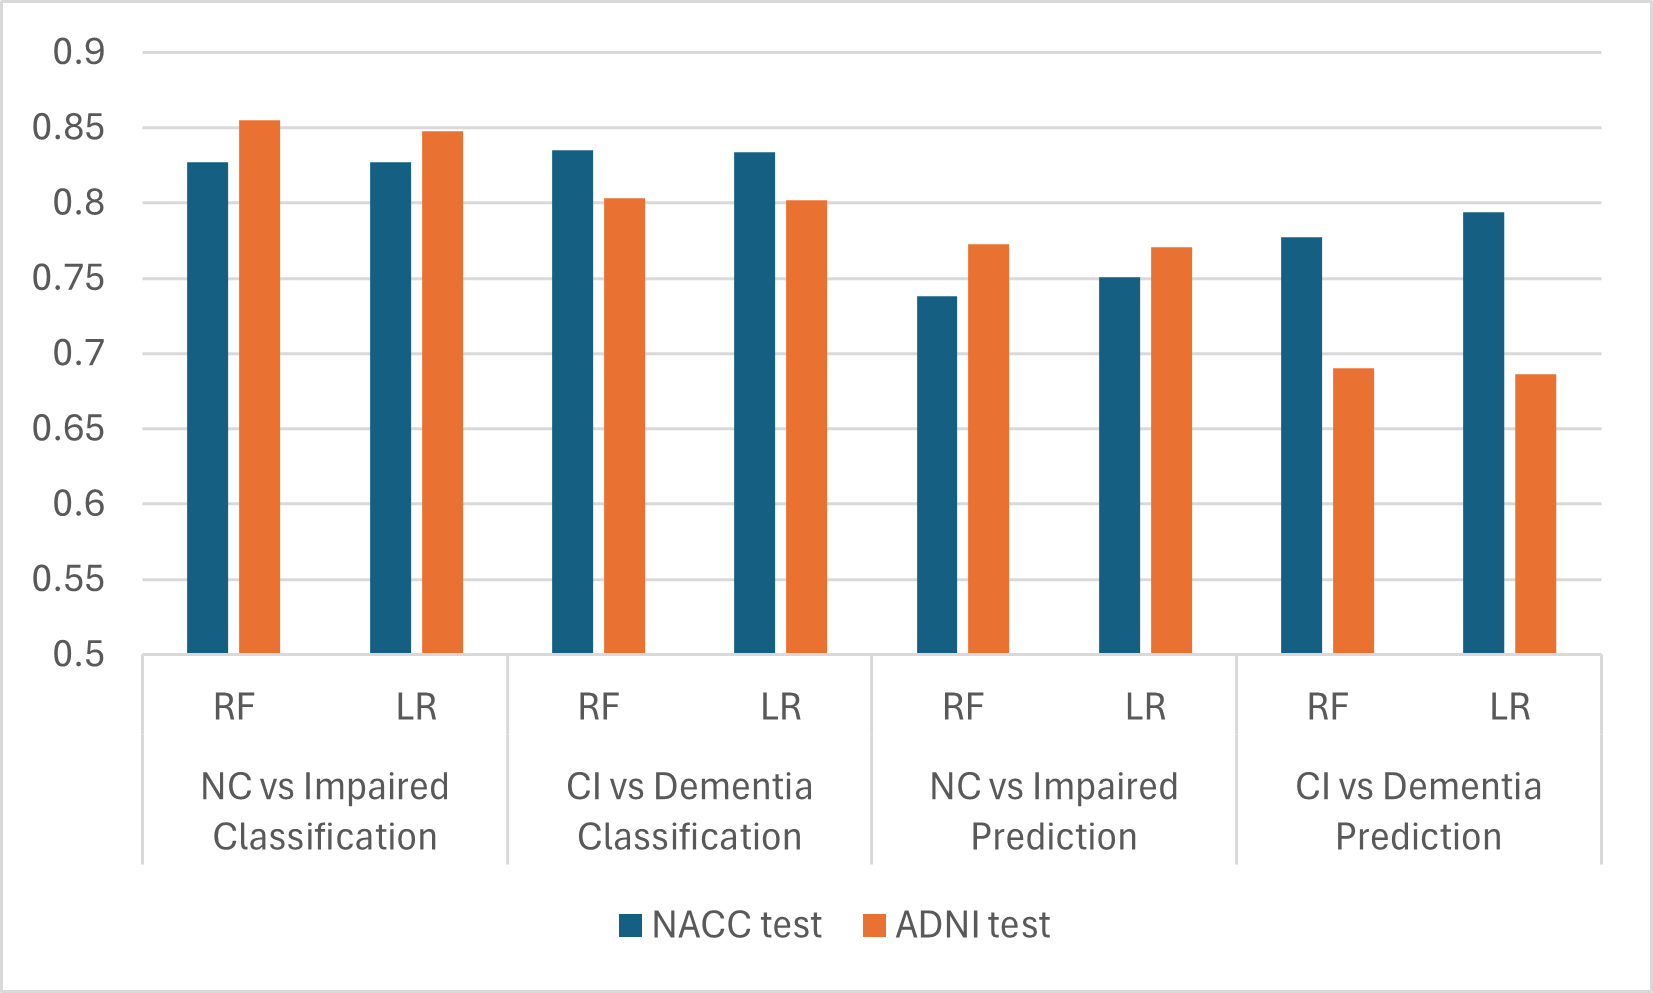
\includegraphics[width=\columnwidth]{figures/generalizability-test.png}
    \caption{Comparison of models performance in NACC and ADNI test data for different classification tasks.}
    \label{fig:nacc-adni-test-compare}
\end{figure}

For the NC vs. Impaired classification, both models showed an increase in F1-score on the ADNI data (RF: 0.827 to 0.855; LR: 0.827 to 0.848). This was driven by a substantial increase in specificity, while the recall experienced a slight drop. This suggests that the models were better at correctly identifying the majority class (NC) in the ADNI dataset, but were less effective at identifying the minority class (Impaired) compared to the NACC test set.

A similar pattern was observed in the NC vs. Impaired prediction task. The F1-scores increased slightly for both models on the ADNI data, with a significant gain in specificity and a decrease in recall. For example, the specificity for the LR model jumped from 0.802 in the NACC test to 0.902 in the ADNI test, while its recall dropped from 0.756 to 0.672. This indicates that the models' ability to correctly predict individuals who would remain healthy was stronger on the ADNI data, but they were less accurate in predicting those who would become impaired.

In contrast, the CI vs. Dementia prediction task saw a decrease in F1-score for both models on the ADNI dataset (RF: 0.777 to 0.690; LR: 0.794 to 0.686). This decline was primarily due to a drop in recall. However, both models showed a more balanced performance in the CI vs. Dementia classification task, with the RF model maintaining a high recall (0.87) on the ADNI data and the LR model maintaining a high specificity (0.862). This difference highlights the difficulty of predicting future cognitive status compared to classifying current ones.

Overall, the models showed solid generalizability, with the prediction tasks proving to be the most challenging for both models and datasets. The models' ability to classify present conditions was more stable and consistent across the NACC and ADNI test sets. The LR model consistently performed well on the prediction tasks, while the RF model was better on some classification tasks. This suggests that both models are valuable, but their strengths lie in different areas.


\section{Model Explainability}
